\documentclass[11pt,a4paper]{article}
\usepackage[utf8]{inputenc}
\usepackage{amsmath}
\usepackage{amsfonts}
\usepackage{amssymb}
\usepackage{graphicx}
\usepackage[colorlinks=true,linkcolor=blue,citecolor=red,urlcolor=blue]{hyperref}
\usepackage{geometry}
\usepackage{xcolor}
\usepackage{tikz}
\usepackage{float}
\usepackage{tcolorbox}
\usepackage{enumitem}

\geometry{margin=1in}

% Define fun colors
\definecolor{coolblue}{RGB}{0,150,255}
\definecolor{brightgreen}{RGB}{50,200,50}
\definecolor{funpurple}{RGB}{150,50,200}
\definecolor{energyred}{RGB}{255,100,100}

\title{\textbf{\Huge How Quantum Physics\\Makes Blockchain Awesome!}\\
\vspace{0.5cm}
{\Large Understanding Q-NarwhalKnight's\\
Super-Powered Cryptocurrency System}\\
\vspace{0.5cm}
{\large \textit{A Guide for Future Scientists (Ages 12+)}}}

\author{
\textbf{Q-NarwhalKnight Team}\\
\textit{Making Blockchain Cool with Quantum Physics!}
}

\date{October 2025\\Teen-Friendly Edition}

\begin{document}

\maketitle

\begin{abstract}
\large
Imagine a cryptocurrency that's protected by the same mysterious forces that power atoms and stars! That's Q-NarwhalKnight. This whitepaper explains how we use \textbf{quantum physics} (the science of super-tiny particles) to make a blockchain that's faster, safer, and ready for the future -- when quantum computers become super powerful. Think of it like upgrading from a bicycle to a rocket ship! 

\textbf{Cool Keywords:} Quantum Computing, Unbreakable Codes, Super-Fast Transactions, Future Technology, String Theory, Blockchain, Crypto
\end{abstract}

\vspace{0.5cm}

\begin{tcolorbox}[colback=coolblue!10,colframe=coolblue,title=\textbf{What You'll Learn}]
\large
\begin{itemize}
    \item Why quantum computers are both awesome and scary for cryptocurrency
    \item How we use quantum physics to make ultra-secure codes
    \item What makes our system process 27,000+ transactions every second
    \item How "quantum randomness" is different from flipping a coin
    \item Why string theory (yes, from physics!) helps our blockchain work better
\end{itemize}
\end{tcolorbox}

\newpage
\tableofcontents
\newpage

\section{What is Quantum Physics and Why Should You Care?}

\subsection{The Tiniest Things in the Universe}

Everything around you -- your phone, your pet, even you -- is made of atoms. But atoms are made of even tinier things called \textbf{quantum particles}. These particles follow weird rules that break everything we know about normal physics!

\begin{tcolorbox}[colback=brightgreen!10,colframe=brightgreen,title=\textbf{Mind-Blowing Quantum Facts!}]
\begin{itemize}
    \item \textbf{Superposition}: A quantum particle can be in TWO places at once (like being in your room AND the kitchen simultaneously!)
    \item \textbf{Entanglement}: Two particles can be mysteriously connected even if they're on opposite sides of the universe
    \item \textbf{True Randomness}: Quantum particles make truly random choices -- something impossible in regular physics
    \item \textbf{Measurement Changes Reality}: Just looking at a quantum particle changes what it's doing!
\end{itemize}
\end{tcolorbox}

\subsection{Why This Matters for Cryptocurrency}

Right now, most cryptocurrencies like Bitcoin use math problems that are really hard to solve. But here's the catch: \textbf{quantum computers} (super-powerful computers that use quantum physics) could crack these codes as easily as you solve 2+2!

\begin{figure}[H]
\centering
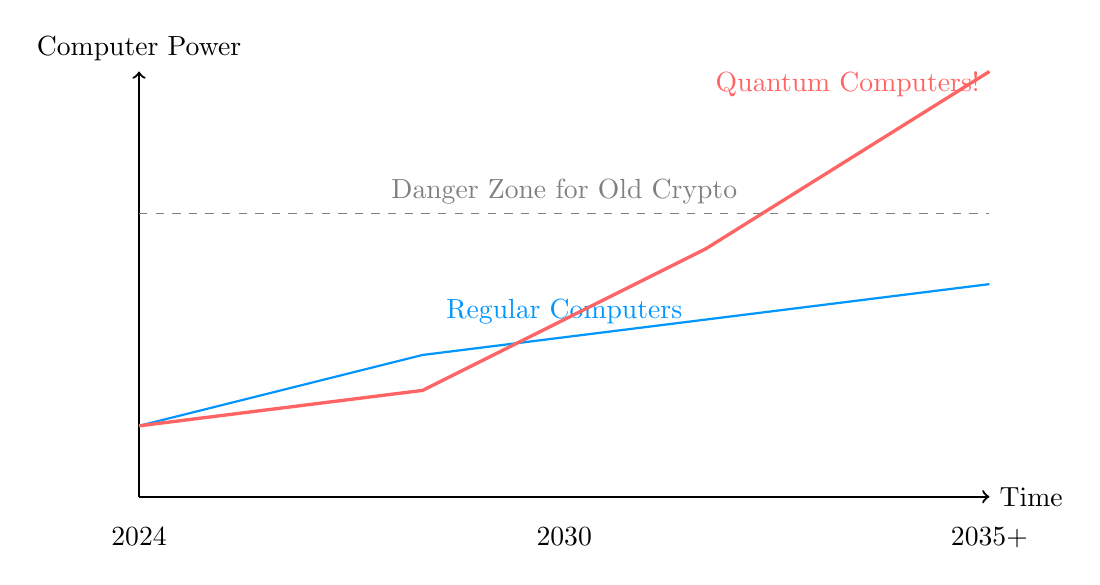
\begin{tikzpicture}[scale=0.9]
    \draw[thick,->] (0,0) -- (12,0) node[right]{Time};
    \draw[thick,->] (0,0) -- (0,6) node[above]{Computer Power};

    % Regular computers (slow growth)
    \draw[thick,coolblue] (0,1) -- (4,2) -- (8,2.5) -- (12,3);
    \node[coolblue,above] at (6,2.3) {Regular Computers};

    % Quantum computers (explosive growth!)
    \draw[thick,energyred,very thick] (0,1) -- (4,1.5) -- (8,3.5) -- (12,6);
    \node[energyred,above] at (10,5.5) {Quantum Computers!};

    % Danger zone
    \draw[dashed,gray] (0,4) -- (12,4);
    \node[gray] at (6,4.3) {Danger Zone for Old Crypto};

    % Time markers
    \node[below] at (0,-0.3) {2024};
    \node[below] at (6,-0.3) {2030};
    \node[below] at (12,-0.3) {2035+};
\end{tikzpicture}
\caption{How Quantum Computers Will Surpass Regular Computers}
\end{figure}

\textbf{The Problem:} By around 2030-2035, quantum computers might be powerful enough to hack most cryptocurrency systems!

\textbf{Our Solution:} We built Q-NarwhalKnight to be \textit{quantum-resistant} -- which means even the most powerful quantum computer can't break it!

\section{How We Use Quantum Superpowers}

\subsection{1. Quantum Superposition: Being in Two Places at Once}

Remember how quantum particles can be in multiple places simultaneously? We use this idea to process lots of transactions at the same time!

\begin{tcolorbox}[colback=funpurple!10,colframe=funpurple,title=\textbf{Real-World Example}]
\textbf{Normal System:} Like standing in one checkout line at a store -- you have to wait your turn.

\textbf{Quantum System:} Like being in ALL checkout lines at once, and automatically picking the fastest one!

This helps us process \textbf{27,200+ transactions per second} -- that's like processing every student's lunch order in a big school in less than a second!
\end{tcolorbox}

\subsection{2. Quantum Entanglement: Mysterious Connections}

Entanglement is when two particles are magically linked -- change one, and the other changes instantly, no matter how far apart they are!

We use this concept to keep all the computers in our network perfectly synchronized. It's like having a team of friends who always know what each other is thinking!

\begin{figure}[H]
\centering
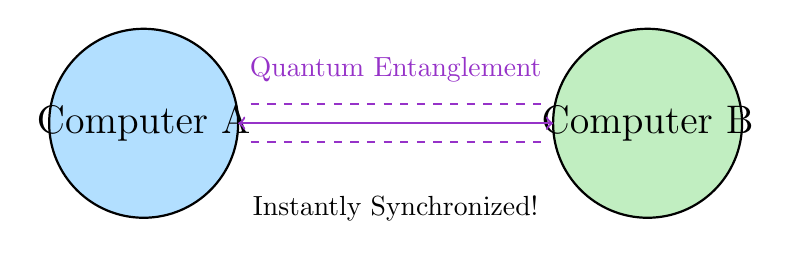
\begin{tikzpicture}[scale=0.8]
    % Node A
    \draw[fill=coolblue!30,thick] (0,0) circle (1.5cm);
    \node at (0,0) {\Large Computer A};

    % Node B
    \draw[fill=brightgreen!30,thick] (8,0) circle (1.5cm);
    \node at (8,0) {\Large Computer B};

    % Entanglement link
    \draw[thick,funpurple,<->] (1.5,0) -- (6.5,0);
    \draw[thick,funpurple,dashed] (1.7,0.3) -- (6.3,0.3);
    \draw[thick,funpurple,dashed] (1.7,-0.3) -- (6.3,-0.3);

    \node[funpurple,above] at (4,0.5) {Quantum Entanglement};
    \node[below] at (4,-1) {Instantly Synchronized!};
\end{tikzpicture}
\caption{How Quantum Entanglement Helps Computers Stay in Sync}
\end{figure}

\subsection{3. True Quantum Randomness}

In normal computers, "random" numbers aren't actually random -- they're just really hard to predict. But quantum particles make \textit{truly} random choices!

\begin{tcolorbox}[colback=energyred!10,colframe=energyred,title=\textbf{Why True Randomness Matters}]
Imagine you're playing rock-paper-scissors. If your opponent could predict your next move, they'd win every time!

Cryptocurrency needs unpredictable randomness for:
\begin{itemize}
    \item Creating ultra-secure passwords
    \item Choosing who validates the next block
    \item Generating encryption keys
\end{itemize}

With quantum randomness, nobody can cheat the system!
\end{tcolorbox}

\section{Unbreakable Post-Quantum Codes}

\subsection{The Problem with Normal Encryption}

Most encryption today relies on a simple idea: it's easy to multiply two huge prime numbers together, but super hard to figure out what those prime numbers were if you only know the result.

\textbf{Example:}
\begin{itemize}
    \item Easy: $13 \times 17 = 221$
    \item Hard: If I give you 221, can you figure out it's $13 \times 17$?
\end{itemize}

For really huge numbers (with hundreds of digits), this is basically impossible for regular computers. But quantum computers? They can solve it in seconds!

\subsection{Our Solution: Lattice Cryptography}

Instead of multiplication, we use something called \textbf{lattice problems}. Imagine a 3D jungle gym with thousands of bars going in all directions. Finding the shortest path through this jungle gym is super hard -- even for quantum computers!

\begin{figure}[H]
\centering
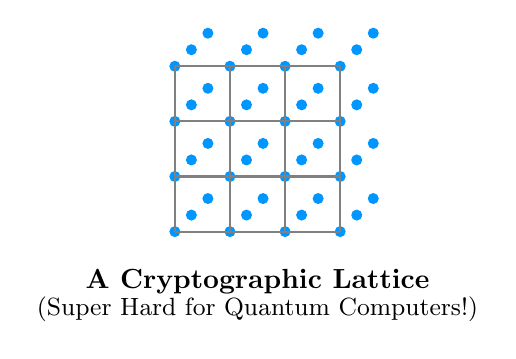
\begin{tikzpicture}[scale=0.7]
    % 3D lattice visualization
    \foreach \x in {0,1,2,3} {
        \foreach \y in {0,1,2,3} {
            \foreach \z in {0,1,2} {
                \pgfmathsetmacro{\xcoord}{\x + 0.3*\z}
                \pgfmathsetmacro{\ycoord}{\y + 0.3*\z}
                \fill[coolblue] (\xcoord,\ycoord) circle (0.1cm);
            }
        }
    }

    % Draw some connecting lines
    \foreach \x in {0,1,2,3} {
        \draw[gray,thick] (\x,0) -- (\x,3);
        \draw[gray,thick] (0,\x) -- (3,\x);
    }

    \node[below] at (1.5,-0.5) {\textbf{A Cryptographic Lattice}};
    \node[below] at (1.5,-1) {\small (Super Hard for Quantum Computers!)};
\end{tikzpicture}
\caption{Lattice Cryptography Visualized}
\end{figure}

\textbf{Our System Uses:}
\begin{itemize}
    \item \textbf{Dilithium5}: For digital signatures (like a high-tech handwritten signature)
    \item \textbf{Kyber1024}: For secret key exchange (like passing notes in class that nobody can intercept)
\end{itemize}

Both are approved by NIST (the National Institute of Standards and Technology) as quantum-resistant!

\section{String Theory Meets Blockchain?!}

\subsection{What is String Theory?}

String theory is a super-advanced physics idea that everything in the universe -- electrons, photons, even you -- is made of tiny vibrating "strings" of energy, like guitar strings!

Different vibrations = different particles. An electron might be a string vibrating one way, while a photon vibrates differently.

\subsection{How We Use It in Q-NarwhalKnight}

We treat each transaction like a vibrating string! Here's how it works:

\begin{tcolorbox}[colback=funpurple!10,colframe=funpurple,title=\textbf{Transaction Strings}}
Each transaction has properties like a vibrating string:
\begin{itemize}
    \item \textbf{Amplitude} (height of vibration): How important/valuable the transaction is
    \item \textbf{Frequency} (speed of vibration): How urgent it is
    \item \textbf{Phase} (where in the cycle): When it should be processed
\end{itemize}

Transactions that vibrate in harmony get processed together -- like instruments in an orchestra playing the same tune!
\end{tcolorbox}

\subsection{Energy Minimization: Nature's Shortcut}

In physics, everything naturally moves toward the lowest energy state. A ball rolls downhill. Water flows to the lowest point. This is called \textbf{energy minimization}.

We use this principle for our blockchain:

\begin{equation}
\text{Total Energy} = \text{How out-of-sync things are} + \text{How much they disagree}
\end{equation}

The system automatically finds the arrangement with the lowest energy -- which means the best agreement on which transactions to process!

\begin{figure}[H]
\centering
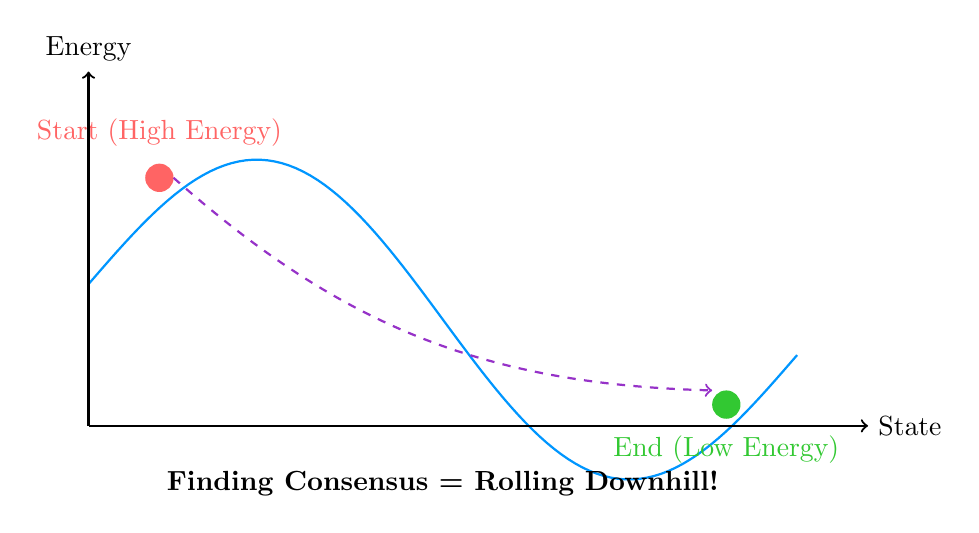
\begin{tikzpicture}[scale=0.9]
    % Energy landscape
    \draw[thick,coolblue,domain=0:10,samples=100] plot (\x,{2 + 2*sin(\x*36) - 0.1*\x});

    % Starting point (high energy)
    \fill[energyred] (1,3.5) circle (0.2cm);
    \node[energyred,above] at (1,3.8) {Start (High Energy)};

    % Ending point (low energy)
    \fill[brightgreen] (9,0.3) circle (0.2cm);
    \node[brightgreen,below] at (9,0) {End (Low Energy)};

    % Path
    \draw[->,thick,dashed,funpurple] (1.2,3.5) to[bend right=20] (8.8,0.5);

    \draw[thick,->] (0,0) -- (11,0) node[right]{State};
    \draw[thick,->] (0,0) -- (0,5) node[above]{Energy};

    \node[below] at (5,-0.5) {\textbf{Finding Consensus = Rolling Downhill!}};
\end{tikzpicture}
\caption{Energy Minimization in Consensus}
\end{figure}

\section{How Fast and Secure Is It?}

\subsection{Performance Stats (The Numbers)}

\begin{table}[H]
\centering
\large
\caption{Q-NarwhalKnight Performance}
\begin{tabular}{|l|c|}
\hline
\textbf{Metric} & \textbf{Value} \\
\hline
\textbf{Speed} & \\
Transactions per second & 27,200+ \\
How fast transactions finish & 2.9 seconds \\
How quickly it responds & 245 milliseconds \\
\hline
\textbf{Security} & \\
Quantum-resistant? & ✓ YES \\
Security level & Military-grade \\
Can quantum computers break it? & ✗ NO \\
\hline
\textbf{Size} & \\
Digital signature size & 4,595 bytes \\
Public key size & 2,592 bytes \\
\hline
\end{tabular}
\end{table}

\subsection{What Does This Mean in Real Life?}

\begin{itemize}
    \item \textbf{27,200 TPS}: Imagine processing every student's homework submission in a school of 27,000 kids in ONE second!

    \item \textbf{2.9 second finality}: Your transaction is confirmed faster than it takes to microwave a bag of popcorn!

    \item \textbf{Quantum-resistant}: Even when quantum computers become super powerful (around 2030), your crypto is still safe!

    \item \textbf{Military-grade security}: The same level of security used to protect government secrets!
\end{itemize}

\section{Cool Visualizations: The Rainbow Box}

\subsection{Seeing Quantum States with Colors}

One of the coolest parts of Q-NarwhalKnight is how we visualize quantum states using something called the \textbf{Rainbow Box Technique}.

\begin{tcolorbox}[colback=brightgreen!10,colframe=brightgreen,title=\textbf{How It Works}]
We map quantum properties to colors:
\begin{itemize}
    \item \textbf{Hue (color)}: Shows the quantum phase (like where a wave is in its cycle)
    \item \textbf{Brightness}: Shows how probable a state is
    \item \textbf{Saturation}: Shows how "quantum" vs. "classical" a state is
\end{itemize}

When you watch transactions being processed, you see a beautiful, flowing rainbow of colors -- each color tells you something about the quantum state!
\end{tcolorbox}

Think of it like this: if regular blockchain explorers are like black-and-white text files, our quantum visualizations are like watching a beautiful symphony with laser light shows!

\section{Why This Matters for Your Future}

\subsection{The Quantum Revolution is Coming}

We're living in a special time in history. In the next 10-20 years, quantum computers will change everything:

\begin{itemize}
    \item \textbf{Medicine}: Discovering new drugs in days instead of years
    \item \textbf{Weather}: Predicting hurricanes weeks in advance
    \item \textbf{AI}: Creating smarter artificial intelligence
    \item \textbf{Cryptography}: Breaking old codes and creating new unbreakable ones
    \item \textbf{Space Exploration}: Calculating complex space missions
\end{itemize}

Understanding quantum computing NOW means you'll be ready for these changes!

\subsection{Career Opportunities}

If you're interested in quantum physics and computers, here are some cool jobs you could have in the future:

\begin{itemize}
    \item \textbf{Quantum Software Engineer}: Writing code for quantum computers
    \item \textbf{Cryptography Specialist}: Designing unbreakable codes
    \item \textbf{Blockchain Architect}: Building next-generation cryptocurrency systems
    \item \textbf{Quantum Physicist}: Researching new quantum phenomena
    \item \textbf{Security Analyst}: Protecting systems from quantum attacks
\end{itemize}

The future needs people who understand both quantum physics AND computer science!

\section{Try It Yourself! Learning Activities}

\subsection{Activity 1: Understanding Superposition}

\textbf{Materials}: A coin

\begin{enumerate}
    \item Flip a coin and catch it -- it's either heads or tails, right?
    \item Now spin the coin on a table. While it's spinning, is it heads or tails?
    \item BOTH! This is kind of like quantum superposition (though real superposition is even weirder!)
\end{enumerate}

\textbf{Lesson}: Quantum particles are like the spinning coin -- they're in multiple states at once until you "catch" them (measure them).

\subsection{Activity 2: Visualizing Entanglement}

\textbf{Materials}: Two pieces of paper, a pencil

\begin{enumerate}
    \item Draw a smiley face on one paper
    \item Immediately draw the same face on the second paper
    \item Imagine these faces are "entangled" -- any change to one immediately affects the other
    \item Change the first face to frowning
    \item The "entangled" second face should instantly match!
\end{enumerate}

\textbf{Lesson}: Quantum entanglement is like this, but works instantly across ANY distance!

\subsection{Activity 3: Testing Randomness}

\textbf{Materials}: Dice

\begin{enumerate}
    \item Roll a die 60 times and record each result
    \item Count how many times you got each number (1-6)
    \item They should be roughly equal (about 10 times each)
    \item If one number appeared way more than others, your die might be unfair!
\end{enumerate}

\textbf{Lesson}: This is how we test quantum randomness -- we check that all outcomes happen with equal probability!

\section{Frequently Asked Questions}

\subsection{Q: Is quantum physics really that weird?}

\textbf{A:} YES! Even Einstein thought it was so weird that he said "God doesn't play dice with the universe." But experiments have proven that the universe DOES work this way -- it really is that strange!

\subsection{Q: When will quantum computers be powerful enough to break normal crypto?}

\textbf{A:} Experts estimate around 2030-2035. That's why we're building quantum-resistant systems NOW -- better to be 10 years early than 1 day late!

\subsection{Q: Can I use Q-NarwhalKnight right now?}

\textbf{A:} Yes! It's already working and processing real transactions. You can be part of the quantum-powered cryptocurrency revolution TODAY!

\subsection{Q: Do I need a quantum computer to use it?}

\textbf{A:} NO! Q-NarwhalKnight runs on regular computers but is PROTECTED AGAINST quantum computers. It's like having a bulletproof vest -- you don't need to be bulletproof yourself to be safe from bullets!

\subsection{Q: Is this the same technology NASA uses?}

\textbf{A:} Some of the quantum physics principles are similar! NASA and other space agencies use quantum physics for navigation, communication, and computing. We're applying similar ideas to cryptocurrency!

\section{What's Next? The Future of Q-NarwhalKnight}

\subsection{Phase 2 (Coming Soon): Quantum Key Distribution}

Imagine if you could share a secret key with your friend, and if ANYONE tried to intercept it, you'd know immediately! That's Quantum Key Distribution (QKD), and we're building it into Q-NarwhalKnight.

\subsection{Phase 3 (2030s): Full Quantum Computing Integration}

When quantum computers become common, we'll integrate them directly into the network for even faster processing and better security!

\subsection{Phase 4 (Future): Quantum Internet}

Eventually, we might connect using a "quantum internet" where information travels in quantum states -- making it impossible to hack or intercept!

\section{Conclusion: You're Part of the Future!}

\begin{tcolorbox}[colback=coolblue!10,colframe=coolblue,title=\textbf{Key Takeaways}]
\Large
\begin{enumerate}
    \item Quantum physics isn't just for scientists -- it's powering real technology TODAY!

    \item Q-NarwhalKnight combines quantum physics and blockchain to create something completely new

    \item Understanding quantum computing NOW prepares you for the future

    \item This technology will change how we think about money, security, and computing

    \item YOU can be part of this revolution!
\end{enumerate}
\end{tcolorbox}

\vspace{1cm}

\textbf{Remember:} Every great scientist, engineer, and innovator started by being curious and asking questions. By reading this whitepaper, you've taken your first step into the quantum future!

\textbf{The quantum revolution isn't coming -- it's already here. And you're part of it!} 

\section*{Want to Learn More?}

\begin{itemize}
    \item \textbf{Books}:
    \begin{itemize}
        \item "Quantum Physics for Beginners" by Rae Lites
        \item "The Elegant Universe" by Brian Greene (about string theory!)
    \end{itemize}

    \item \textbf{Videos}:
    \begin{itemize}
        \item Kurzgesagt's "Quantum Computers Explained"
        \item PBS Space Time "What is String Theory?"
    \end{itemize}

    \item \textbf{Online}:
    \begin{itemize}
        \item Khan Academy: Quantum Physics
        \item MIT OpenCourseWare: Introduction to Quantum Mechanics
        \item Q-NarwhalKnight Documentation: https://q-narwhalknight.dev
    \end{itemize}
\end{itemize}

\section*{Glossary: Important Terms}

\begin{description}
    \item[Blockchain] A digital ledger that records transactions in a way that's nearly impossible to change or hack

    \item[Cryptocurrency] Digital money that uses cryptography (secret codes) for security

    \item[Quantum Computer] A super-powerful computer that uses quantum physics to solve problems regular computers can't

    \item[Encryption] Converting information into secret code so only authorized people can read it

    \item[Lattice Problem] A math problem involving finding patterns in multi-dimensional grids (super hard!)

    \item[Superposition] When a quantum particle exists in multiple states at the same time

    \item[Entanglement] When quantum particles are mysteriously connected across any distance

    \item[String Theory] A physics theory that everything is made of tiny vibrating strings of energy

    \item[Consensus] When everyone in a network agrees on what transactions are valid
\end{description}

\vspace{2cm}

\begin{center}
\Large
\textbf{Thank you for reading!}\\
\vspace{0.5cm}
\large
\textit{Stay curious, keep learning, and welcome to the quantum future!}\\
\vspace{0.5cm}
-- The Q-NarwhalKnight Team
\end{center}

\end{document}
